%
% ****
\chapter{Implementierung des TW-Netzes}
\label{chap:imp}
% ****
%

	Die Implementierung des gesamten neuronalen Netzes inklusive der Simulationsumgebung erfolgt in der Programmiersprache \texttt{Python}. Als Module werden zum einen das bereits vorgestellte Leaky Integrate and Fire - Modell implementiert, zum anderen diverse Algorithmen zur Suche von individuellen Parametern des neuronalen Netzes. Darüber hinaus ist das Programm in der Lage, eine Simulation der gefundenen Parameter durch die Simulationsumgebung \texttt{CartPole\_v0} von OpenAI Gym zu zeigen und Parameter über die Simulationszeit zu plotten. Die Module sowie diverse Dokumentationen und Informationen sind auf meiner GitHub-Repository\footnote{https://github.com/J0nasW/BA} \cite{BA} zu finden.\\
		

% ***
\section{Aufbau des Programms}
\label{sec:imp_module}
% ***
	Ziel dieser Arbeit ist es, das Programm mitsamt allen Modulen und Abhängigkeiten so modular wie möglich aufzubauen. Es soll einen zentralen Punkt zum ändern von Parametern und Laufzeiten geben sowie eine Datei zum steuern der Simulationsläufe und Ergebnisse. Es soll als ein universeller Simulator für biologische, symmetrische neuronale Netze agieren und durch verschiedene graphische Darstellung gute Analysemöglichkeiten bieten. Darüber hinaus wurde jeder Codeabschnitt genauestens kommentiert und durch die Versionierung seitens GitHub nachvollziehbar dokumentiert.\\
	Das Programm beinhaltet folgende Module:\\
	\begin{minipage}{0.35\textwidth}
		\vspace{0.3cm}
		\begin{forest}
			pic dir tree,
			where level=0{}{% folder icons by default; override using file for file icons
				directory,
			},
			[TW Circuit
				[docs]
				[information]
				[modules
					[inspect.py, file]
					[lif.py, file]
					[parameters.py, file]
					[random\_search\_v2.py, file]
					[visiualize.py, file]
					[weights.py, file]]
				[parameter\_dumps]
				[weight\_dumps]
				[main.py, file]]
		\end{forest}
	\end{minipage}
	\begin{minipage}{0.65\textwidth}
		\begin{itemize}
			\item Der Ordner \texttt{docs} beinhaltet wichtige Dokumentationen bezüglich des Codes und dem Umgang mit diversen Befehlen innerhalb der \texttt{main.py}. Darüber hinaus wird hier ebenfalls diese Arbeit inklusive des \LaTeX-Codes abgelegt.
			\item Aufgrund vieler komplexer Simulationen mit verschiedenen Parametersätzen wurde die Berechnung von Heim- und Unirechnern auf Rechenzentren ausgelagert. Der Ordner \texttt{information} wird genutzt, um Informationen über jede Simulation (Ergebnisse, Zeitstempel, Zugehörigkeit, ...) im Form einer TXT-Datei zu speichern.
			\item Alle nötigen Module zur Simulation und Visualisierung finden sich in dem Ordner \texttt{modules} wieder. Genauere Informationen zu den einzelnen Skripten werden in den nächsten Sektionen aufgeführt.
			\item parameter\_dumps und weight\_dumps sind die Resultate der Simulationsläufe. In diesen Ordnern werden Parameter und Gewichte des neuronalen Netzes nach erfolgreichen Simulationsläufen abgespeichert. Die Dateien werden durch das Skript \texttt{hickle} in ein HDF-5 Dateiformat gespeichert.
		\end{itemize}		
	\end{minipage}
	
	
		
% ***
\section{Implementierung der Suchalgorithmen}
\label{sec:imp_search}
% ***
	Die Suchalgorithmen befinden sich jeweils in dem Ordner \texttt{modules} und werden durch Import in der Datei \texttt{main.py} aufgerufen. Sie erhalten bei Aufruf die gesetzte Simulationszeit (bspw. 12 Stunden) und bei Bedarf bereits errechnete Parameter. Als Ausgabe wird ein Dump der errechneten Parameter oder Gewichte gespeichert sowie eine Informationsdatei, welche Zugehörigkeiten, Anz. an Simulationen, Laufzeiten und den gesamten Reward enthält.
	
	\subsection{Suchalgorithmus RandomSearch}
		Der Suchalgorithmus RandomSearch wurde direkt in die Simulation eingebunden. Es werden die Parameter $C_m, G_{Leak}, U_{Leak}, \sigma, w, \hat{w}$ durch eine Gleichverteilung in den bereits genannten Grenzen zufällig erzeugt. Um gleichverteilte, zufällige Werte zu erzeugen, wird eine Funktion aus dem bekannten Package \texttt{numpy} verwendet.
		\begin{algorithm}
			\SetKwInOut{Input}{Input}
			\SetKwInOut{Output}{Output}
			
			\Input{Anz. Nervenzellen, Anz. Synapsen, Anz. Gap-Junctions}
			\Output{Arrays $C_m, G_{Leak}, U_{Leak}, \sigma, w, \hat{w}$}
				\tcp{Generieren von Zufallsvariablen durch Gleichverteilung.}
				\tcp{Für Nervenzellen:}
				$C_m$ = np.random.uniform(low = 0.01, high = 1, size = (1,Anz. Nervenzellen))\\
				$G_{leak}$ = np.random.uniform(low = 0.05, high = 5, size = (1,Anz. Nervenzellen))\\
				$U_{leak}$ = np.random.uniform(low = -70, high = 0, size = (1,Anz. Nervenzellen))\\
				\tcp{Für Synapsen:}
				$\sigma$ = np.random.uniform(low = 0.05, high = 0.5, size = (1,Anz. Synapsen))\\
				$w$ = np.random.uniform(low = 0, high = 3, size = (1,Anz. Synapsen))\\
				$\hat{w}$ = np.random.uniform(low = 0, high = 03, size = (1,Anz. Gap-Junctions))
				\KwRet{$C_m, G_{Leak}, U_{Leak}, \sigma, w, \hat{w}$}	
			\caption{random\_parameters}
		\end{algorithm}
		Nach Aufruf des Algorithmus \texttt{random\_parameters} wird eine Simulation mit den erzeugten Parametern und maximal 200 Zeitschritten durchgeführt. Der Reward dieser Simulation wird mit vergangenen Rewards verglichen. Wenn die Simulation einen Reward größer oder gleich 200 erreicht, gilt die Simulation als erfolgreich, andernfalls wird nach Ablauf der Simulationszeit der Algorithmus unterbrochen.\\
		Der gesamte Programmablauf gestaltet sich vereinfacht wie folgt:
		\begin{algorithm}
			\SetKwInOut{Input}{Input}
			\SetKwInOut{Output}{Output}
			
			\Input{Simulationszeit}
			\Output{Simulationsinformation (information.txt), Parameter-Dump als .hkl Datei}
			
			action = episodes = best\_reward = 0\\
			env = gym.make('CartPole-v0')\\
			\While{True}{
				initialize(Default\_U\_leak)\\
				episodes $\leftarrow$ episodes + 1\\
				$C_m, G_{Leak}, U_{Leak}, \sigma, w, \hat{w}$ = random\_parameters()\\
				reward = run\_episode($C_m, G_{Leak}, U_{Leak}, \sigma, w, \hat{w}$) \tcp*{Simulation mit neuen Parametern - Siehe Sec. \ref{sec:imp_sim}}
				\If{reward $\geq$ best\_reward}{
					Set best\_reward $\leftarrow$ reward
					Result = [$C_m, G_{Leak}, U_{Leak}, \sigma, w, \hat{w}$] \tcp*{Für Parameter-Dump}
					\If{reward $\geq$ 200}{
						\textbf{break}\tcp*{Exit-Argument, wenn Reward von 200 erreicht wurde}
					}
				}
				\If{elapsed\_time $>$ simulation\_time}{
					\textbf{break} \tcp*{Exit-Argument, um genaue Laufzeiten zu erzielen}
				}
			}
			\KwRet{information.txt, parameter\_dump.hkl, date, best\_reward}
			\caption{random\_search\_v2}
		\end{algorithm}
		Die gesamte Berechnung der Synapsenströme sowie Membranpotentiale und die Simulation findet in der Methode \texttt{run\_episode} statt und wird in Sektion \ref{sec:imp_sim} präziser erläutert.
	\subsection{Suchalgorithmus Weights}
		Als erstes Optimierungsverfahren nach erfolgreicher Simulation der Parameter des neuronalen Netzes wird nun der Algorithmus Weights eingesetzt. Dieser lädt die bereits simulierten Parameter und gewichtet jede Synapse mit einem Faktor $g\in[0,1]$. Somit wird schnell festgestellt, welche Synapsen bei dieser Simulation elementar sind und ob andere gar weg gelassen werden können. Durch diese Simulation war es möglich, das in Kap. \ref{chap:neuro} vorgestellte symmetrische Neuronale Netz (Abb. \ref{fig:nn_new}) zu entwickeln. Die dort gezeigten Synapsen werden lediglich leicht gewichtet und sind somit wichtig für den Erfolg des neuronalen Netzes.\\
		Der Gewichtungsalgorithmus ist rechenintensiver als RandomSearch, da insgesamt 16 Synapsen bzw. Gap-Junctions pro Episode mit zufällig gewählten Gewichten versehen werden, um den Reward zu steigern. Jedoch wird ein im Schnitt um das Dreifache höherer Reward verzeichnet bei gleichbleibenden Parametern, was einer enormen Optimierung gleichkommt.\\
		Aufgerufen wird dieser Algorithmus gleich wie RandomSearch aus der \texttt{main.py}-Datei. Als Input werden die bereits errechneten optimalen Parameter der jeweiligen Nervenzellen und Synapsen eingegeben sowie die maximale Simulationszeit. Ebenfalls gleich dem Algorithmus RandomSearch produziert Weights einen Parameter-Dump, welcher die errechneten Gewichte enthält sowie eine Informationsdatei im \texttt{.txt}-Format, welche weitere Zugehörigkeitsinformationen sowie die Anzahl an Simulationen und die Dauer enthält.
		
	\subsection{Simulation in der Google Cloud Platform\textsuperscript{\textregistered}}
		Wie bereits in diesem Abschnitt mehrfach erwähnt, sind die implementierten Suchalgorithmen RandomSearch und Weights äußerst rechenintensiv. Beide Skripte erfordern das zufällige Generieren einer hohen Anzahl an Parametern sowie die Anwendung dieser Parameter auf das gegebene Problem durch numerische Lösungsansätze \ref{sec:lif_imp}. Darüber hinaus müssen Parameter zwischengespeichert und Dumps auf Festplatten geschrieben werden. Darüber hinaus wird für eine erfolgreiche Simulation des inversen Pendels ein Parametersatz mit hohem Reward gefunden werden, um eine korrekte Funktionsweise des neuronalen Netzes zu gewährleisten.\\
		Bei dem in Abb. \ref{fig:nn_new} gezeigten Netz werden die Parameter $C_m, G_{Leak}, U_{Leak}, \sigma, w, \hat{w}$ für Synapsen, Gap-Junctions und Nervenzellen simuliert.
		\begin{center}
			\begin{tabular}{c@{\hskip 0.5cm}c@{\hskip 0.5cm}c@{\hskip 0.5cm}}    \toprule
				\setlength{\tabcolsep}{50pt}
				\renewcommand{\arraystretch}{1.5}
				\emph{Parameter}	& \emph{Kategorie}  & \emph{Anzahl} \\\midrule
				$C_m$				& Nervenzelle		& 4				\\ 
				$G_{Leak}$	 		& Nervenzelle		& 4				\\
				$U_{Leak}$	 		& Nervenzelle		& 4				\\
				$\sigma$			& Synapse			& 16			\\
				$w$					& Synapse			& 16			\\ 
				$\hat{w}$			& Synapse			& 2				\\\bottomrule
				Gesamt:				&					& \textbf{46}	\\
				\hline
			\end{tabular}
		\end{center}
		Somit werden in jedem Simulationslauf zuerst \textbf{46} Parameter in gegebenen Grenzen durch eine Gleichverteilung erzeugt und anschließend durch das \texttt{compute}-Modul \ref{sec:lif_imp} die benötigten Synapsenströme und Membranpotentiale errechnet.\\
		Das Modul Weights erzeugt, ähnlich RandomSearch, zuerst für jede Synapse und Gap-Junction ein gleichverteiltes, zufälliges Gewicht $g\in[0,1]$. Somit werden insgesamt \textbf{10} Gewichte pro Episode erzeugt und auf das Modell angewendet. Um die erforderlichen Ströme und Potentiale zu errechnen, wird das \texttt{compute}-Modul um die Funktion der Gewichtung erweitert.\\
		Ein solches Simulationsvorhaben wird üblicherweise nicht mehr auf dem Heimrechner laufen gelassen, sondern findet den Weg in die Cloud. Gerade in den letzten Jahren haben Cloud-Computing-Firmen wie Amazon mit AWS, Microsoft mit der Azure Cloud und Google mit der Google Cloud Platform (GCP) an großer Aufmerksamkeit gewonnen. Die einfache Handhabung und Kontrolle über eigene virtuelle Instanzen von ganzen Betriebssystemen erlaubt eine zuverlässige und effiziente Simulation von Parametern. In dieser Angelegenheit wurde sich für die Google Cloud Platform entschieden, da diese ein sehr gutes User Inferface hat und kostengünstige, virtuelle Maschinen anbietet. Gemietet wurde ein Server mit dem Standort Frankfurt, welcher über vier virtuelle Intel XEON\textsuperscript{\textregistered} Prozessoren sowie 12GB DDR4 Arbeitsspeicher verfügt. Dies erlaubt eine schnelle Simulation von vier Instanzen zur gleichen Zeit sowie den Vorteil, das Langzeitsimulationen von 12 Stunden oder mehr im Hintergrund oder über Nacht erfolgen können.\\
		Auf der virtuellen Instanz wurde ein Linux Ubuntu 18.04 LTS installiert und bereitgestellt. Dazu wurde die vorbereitete GitHub Repository \cite{BA} auf das System geklont und die benötigten Pakete installiert. Durch einen Cronjob ausgeführt durch \texttt{crontab -e} wird die Simulation zu einer festen Uhrzeit gestartet und für jeweils 12 Stunden ausgeführt.
		\begin{figure}[!h] %[!t] ...
			\centering
			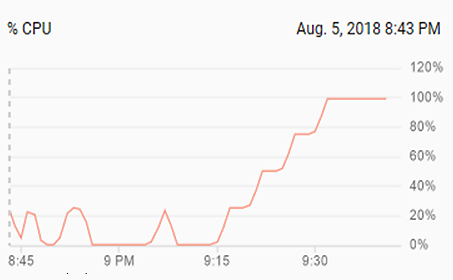
\includegraphics[width=5cm]{figures/chap_implement/GCP.png}
			\caption{Systemauslastung der virtuellen Instanz auf der GCP}
			\label{fig:gcp_1}
		\end{figure}\\
		Wie in Abb. \ref{fig:gcp_1} zu sehen, werden die Suchalgorithmen nacheinander durch den Cronjob ausgeführt, da pro Suchlauf nur ein Prozessorkern in Anspruch genommen werden kann. Der virtuelle Prozessor erreicht somit bei vier gleichzeitigen Simulationsläufen eine Auslastung von $100\%$.\\
		Die Ergebnisse der Suchläufe werden in Form von Parameter- und Weight-Dumps via einem Apache Webserver bereitgestellt und können problemlos auf dem Heimrechner visualisiert werden. Diese Methode funktioniert darüber hinaus auch Plattform- und Versionsübergreifend. Eine Simulation kann Dumps mit Python 2.7 erstellen, welche durch einen Heimrechner mit Python 3.6 visualisiert werden können.

% ***
\section{Simulationsumgebung: OpenAI Gym}
\label{sec:imp_sim}
% ***
	main.py
	OpenAI Gym

% ***
\section{Visualisierung und Auswertung}
\label{sec:imp_vis}
% ***
	visiualize.py
	\begin{algorithm}
		\SetKwInOut{Input}{Input}
		\SetKwInOut{Output}{Output}
		
		\Input{$u, u_{rest}, t, \vartheta, R, C, I_0$}
		\Output{Array $u(t)$ mit $t=1,2,3,...$}
		
		\For{$i\leftarrow 0$ \KwTo $t_{max}$}{
		\emph{$i$ als Zähl-Variable}\\
			\eIf{$u \leq \vartheta$}{
				\tcc{Aufaddieren, bis der Threshold $\vartheta$ erreicht ist}
				Berechne momentane Spannung $u$ bei $t=i$\\
				Erweitere das Array $u_{array}$ um aktuelle Spannung $u$
				i hochzählen $i += 1$
			}{
				\tcc{Treshold $\vartheta$ ist erreicht, setze $u$ auf $0$ zurück}
				$i = 0$
				Berechne momentane Spannung $u$ bei $t=0$\\
				Erweitere das Array $u_{array}$ um aktuelle Spannung $u$
				i hochzählen $i += 1$
			}	
		}
		\KwRet{$u_{array}$}
		
		\caption{Das LIF-Modell}
	\end{algorithm}

% ***
\section{Sonstige Implementierung}
\label{sec:imp_vis}
% ***
	inspect.py
	parameters.py
	parameter und weight dumps + hickle

% ***
\section{Steuerung und Zusammenfassung}
\label{sec:imp_zusammenfassung}
% ***

%%% Local Variables: 
%%% mode: latex
%%% TeX-master: "main"
%%% End: 
